% Chapter Template

\chapter{The Use of Semi-supervised Learning in Classification of English Grammatical Structures} % Main chapter title

\label{Chapter2} % Change X to a consecutive number; for referencing this chapter elsewhere, use \ref{ChapterX}

\section{Introduction}

Common European Framework Reference (CERF) is a standard for describing language achievement on a six-point scale, from A1 for beginners, up to C2 for proficient user ability on the four primary skills reading, writing, listening, speaking, and the two secondary skills: vocabulary and grammar. The latter two skills are considered the backbone for the four primary skills in terms of difficulty. For example, frequently uncommon lexical item like \emph{sagacious} makes the sentence in which it appears more difficult to an English learner than a sentence with a more frequent lexical item like \emph{wise}. Similarly, grammatical structures also play a vital role in the overall difficulty of a sentence. For instance, the word \emph{should} conveys different meaning in \emph{I should study for my final exams.} than in \emph{This is your mission should you accept it.}. The latter is considered more difficult to an English learner because the use of \emph{should} as a conditional is less frequent than its use as a modal auxiliary expressing necessity. 

With the rapid development of Wide World Web and social media, countless number of digital texts and video materials can be harnessed for language learning and teaching[@cite authentic material]. However, deciding the appropriateness of materials to learners is very labor-intensive task for English teachers. Instructors spent hours sifting through materials online to determine their difficulty and whether or not they are appropriate for their learners. To this end, we leverage the power of machine learning to build a tool that can automatically determine the difficulty of a given text according to CEFR guidelines. 
CEFR provides 1200 criteria \citep{noauthor_english_nodate} for the difficutly of grammatical structures \ref{tab:cefr}.
\begin{table}
\caption{An excerpt of English sentences and their corresponding CEFR difficulty levels}
\centering
\begin{tabular}{l|c|c|c}
Sentence   & Level \\
\hline
I go there every year with my friends & A1 & \\
I think swimming is good for my body. & A2 & \\
Tomorrow I'm expecting a delivery of our latest\\ catalogues. & B1 & \\
Do not hesitate to contact me should \\you need further information. & B2 & \\
Living in Greece, I have had a chance \\to realise how much tourism can affect one's life. & C1 & \\
There were no photographs of \\him in Ann 's mother's albums. & C2 & \\
\end{tabular}
\label{tab:cefr}
\end{table}

We treat this task as a multinomial classification problem. In our first attempt, we train a logistic regression classifier optimized by Newton-Raphson method on a dataset of around 3000 examples provided by [englishprofile.com], described in details in section 2. We get F1 score of 0.67. In our second attempt, we use the trained classifier from our first attempt to predict the difficulty of sentences in an unlabeled corpus to fetch more training. After that, we merge the newly fetched data with the original dataset (obtained from Englishprofile.com) and re-train another multinomial logistic regression classifier from scratch to get F1 score of 0.79. 

\section{Related Works}
\label{sec:research_background}

Sentence classification is the most common task in natural language processing. Considerable number of studies conducted on lexicalized tasks like sentiment analysis, spam filtering, news categorization, etc. Rarely do we see work on classification sentences based on their syntactic structures. Thus, to the best of our knowledge no work has ever tackled the task of classifying the grammatical difficulty of English sentences according to CEFR guidelines. Therefore, we will briefly survey techniques used to solve general sentence classification problems. 

Proximity-based Algorithms such as Rocchio's algorithm \citep{rocchio1971relevance}  and K-nearest neighbor \cite{tam_comparative_2002} build vector for each class using a training set of document by measuring the similarity, such as Euclidean distance or cosine similarity, between the documents. Some studies \cite{bang_hierarchical_2006} incorporated dictionary-based methods to construct a conceptual similarity with KNN classifier, while \cite{chang_using_2009} combine two KNN classifier with a Naive Bayes one using TF-IDF over phrases to categorize large collections of emails. While proximity-based methods perform well on document classification, yet using them on large training set is not feasible as computing similarities across documents is computationally and resource-wise expensive. Another disadvantage is that noise and irrelevant data can severely degrade the performance of the classification.

Another family of classifier that work well in text categories tasks are decision trees. known for their rule-based approach, Decision trees are favored for their high interpretability \cite{apte_towards_1994}. Classification using this method is done through automatic creating of "if-then" rules. Their use in tasks like spam filtering is very common even with the advent of deep neural network methods \cite{wu_behavior-based_2009}. Another common powerful classifier is Naive Bayes that based on Baye's rule. It perform surprisingly well for many real world classification applications under some specific conditions \cite{mccallum_comparison_nodate} \cite{rish_analysis_2001}. While Naive Bayes do not often outperform discriminative classifiers like Support-Vector Machine, it has the advantage of functioning well with small training data. \cite{kim_effective_2006} and \cite{isa_text_2008} show good results by selecting Naive Bayes with SVM for text classification and clustering the documents. Using a Poisson Naive Bayes for text classification model also yield very good results \cite{isa_text_2008}.  
 
The SVM classification method and logistic regression have shown outstanding results when used in text classification tasks \citep{Yang1999ARO} \cite{brucher2002document} perhaps because of their capacity of handling high-dimensional sparse data well.  However,they can be relatively complex in training and require high time and resource consumption.



\section{Method}
\label{sec:logistic}

\subsection{Dataset: English Grammar Profile}
The dataset used for this study, provided by English Grammar Profile, exhibits typical grammar profile for each level. It consists of 3615 examples and 1215 rules, divided as follows: class A has 1194 supporting examples; class B has 1775 examples; and class C has 646 supporting examples. We merged each the six levels into three supercategories in order to provide more data within each category. 

\begin{itemize}
	\item \textbf{Rule}: Can use 'and' to join a limited range of common adjectives.
	\item \textbf{Example}: The teachers are very nice and friendly.
	\item \textbf{Level}: A1
\end{itemize}
As we can see, the dataset provides some guideance of what characterizes each example. Using these rules, one can easily create a set of regular expression rules and solve the problem symbolically. However, using a statistical approach to detect the difficulty class without hand-crafting rule is very challenging as there are not enough examples for each case within each category. Thus, in order to get good results, we are using a semi-supervised data augmentation technique similar to Yarawsky's bootstrapping approach \cite{yarowsky_unsupervised_1995}. 

\begin{figure}[t]
	\centering
    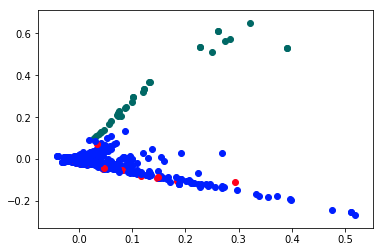
\includegraphics[width=.75\linewidth]{../Figures/pca_proj.png} 
	\caption{2d projection of the three classes A, B and C using K-means Clustering and PCA}
	\label{fig:cmdstudy}
\end{figure}

\subsection{Multinomial Logistic Regression}
Suppose that $\mathbf{x}$ is the vectorized sentence in either of its two forms: BoW or TfIDF, $y\in Y$ is the class label, $\mathbf{w}_k$ and $b_k$ are network parameters associated with class $y$. Then the probability of $\mathbf{x}$ belonging to the class $y$ can be defined by the Softmax function:
\begin{equation}
p(y|\mathbf{x}) =\frac{1}{z(\mathbf{x})}\exp(\mathbf{w}_y^T\mathbf{x}+b_y) \,,
\label{eq:softmax}
\end{equation}
where $z(\mathbf{x}) = \sum_{j=1}^{K}\exp(\mathbf{w}_j^T\mathbf{x}+b_j)$.

Let the log-likelihood function be $$L ( \beta ) = \sum _ { i = 1 } ^ { N } \log p _ { g _ { i } } \left( x _ { i } ; \beta \right)$$. 

$$= \sum _ { i = 1 } ^ { N } \left[ \overline { \beta } _ { g _ { i } } ^ { T } x _ { i } - \log \left( 1 + \sum _ { l = 1 } ^ { K - 1 } e ^ { \overline { \beta } _ { l } ^ { T } x _ { i } } \right) \right]$$

To apply Newton-Raphson method, we need the second derivative of the log likelihood function

$$\frac { \partial ^ { 2 } L ( \beta ) } { \partial \beta _ { k j } \partial \beta _ { m n } } = - \sum _ { i = 1 } ^ { N } x _ { i j } x _ { i n } p _ { k } \left( x _ { i } ; \beta \right) \left[ l ( k = m ) - p _ { m } \left( x _ { i } ; \beta \right) \right]$$

The formula for updating $\beta_{new}$ for multiclass is:
$$\beta ^ { \text { new } } = \beta ^ { \text { old } } + \left( \tilde { \mathbf { X } } ^ { T } \mathbf { W } \tilde { \mathbf { X } } \right) ^ { - 1 } \tilde { \mathbf { X } } ^ { T } ( \mathbf { y } - \mathbf { p } )$$

where $y$ is the concatenated indicator vector of dimension $N \times (K-1)$, $p$ is the concatenated vector of fitted probabilities of dimension $N \times (K-1)$, $\tilde{X}$ is an $N(K-1)\times (p+1)(K-1)$ matrix; and Matrix $W$ is an $N(K-1)\times N(K-1)$ square matrix.

\subsection{Feature Design}

For this task we are comparing two common methods of feature generation in natural language processing and information retrieval: bag-of-word model and term-frequency inverse-document frequency (TFIDF)

\subsubsection{Bag of Word Model} a method to represent the occurrence of words within one sentence. We add different variation by counting unigram, bigram and trigram frequencies. In addition, because this model ignores the order or the location of the word in the sentence, it might not be that helpful to our task as it is not lexicalized and the grammar is core of it. Therefore, we replace some lexical words such as nouns, adjactive with their parts-of-speech tags in order to enforce the presence the of the grammatical category, and avoid the influence of the word itself.  For example, the sentence this is your mission should you accept it” becomes this is NP should S-PRN VRB O-PRN (CLAUSE)”. 

\subsubsection{TF-IDF}  This common information retrieval technique differs from the regular bag-of-words model in that length of the sentence and the frequency of words across sentences does not influence the score of a sentence as it is normalized by other sentences in the dataset. TF·IDF is calculated based on term frequency and document frequency. Term frequency is the number of times a term $t$ occurs in a document $d$ , denoted by TF (t, d) . Document frequency measures the number
of documents in which a term t occurs, denoted by DF(t) . TF·IDF is typically calculated as:

$$T F \cdot I D F ( t , d ) = T F ( t , d ) \cdot \log \frac { | D | } { D F ( t ) }$$, where $|D|$ is the total number of documents.





\section{Experimental Results}
\label{sec:exp}

In this section, we evaluate several variations of our method against random model as our baseline model. In the following experiments, all methods are done using Python 3.5 and Scikit Learn Library, tested on MacBook Pro laptop with Core i5 processor and 8 GB of RAM.

\subsection{First Phase}

In the first phase of our experiment, we train a logistic regression classifier, optimized by Newton-Raphson method , on English Grammar Profile dataset. We also introduce a  feature design method to mask word categories with their part-of-speech tags in order to preserve grammatical information and avoid the lexical influence of the word. We use a combination of feature design methods such as:

\begin{itemize}
	\item \textbf{BoW}: Apply unigram, bigram and trigram bag-of-words model with both word tokens, and masked tokens.
	\item \textbf{Tf-idf}: Apply unigram, bigram and trigram tf-idf model with both word tokens, and masked tokens.
\end{itemize}


\begin{figure}[t]
	\centering
    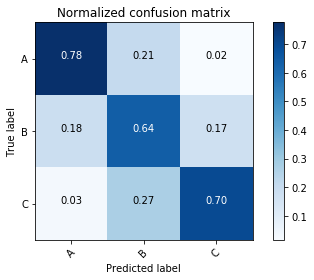
\includegraphics[width=.75\linewidth]{../Figures/conf_matrix_iter1.png} 
	\caption{Confusion matrix illustrating the performance of LR-BoW-Word model with class weight to deal with data imbalance}
	\label{fig:cmdstudy}
\end{figure}

\begin{table}
\centering
\caption {Comparison of Precision-Recall - Phase One}
\begin{tabular}{l|c|c|c}
Model  &  Precision (\%) &  Recall (\%)  & F1 (\%) \\
\hline
Random-Baseline  &  39 (\%) &  39 (\%)  & 39 (\%) \\
\textbf{BoW-LR-Words}  &  70 (\%) &  \textbf{69} (\%)  & \textbf{69} (\%) \\
BoW-LR-Masked  &  66 (\%) &  62 (\%)  & 63 (\%) \\
Tfidf-LR-Words  &  \textbf{75} (\%) &  66 (\%)  & 60 (\%) \\
Tfidf-LR-Masked  &  66 (\%) &  64 (\%)  & 61 (\%) \\
\hline

\end{tabular}
\label {tb:flickre2e}
\end{table}

From table 2, we compare the performance of 4 variations of our method against the baseline, which is a random model. Surprisingly, we notice that our bag-of-words model with word tokens (BoW-LR-Words) outperform the one with masked sequence in terms of precision and recall respectively. It also outperforms (tfidf-LR-words) model in terms of recall only, while the latter has higher recall. From the confusion matrix (fig. 2), we see that (BoW-LR-Words) model predicts most of testing data correctly even though the number of training data is not equal among the classes, especially for class C. Therefore, we needed to assign certain weights to each class during the training in order to avoid this imbalance in the data. 

\subsection{Second Phase}

The results shown in Table 2 does in fact indicate that the linear model has learned the associations between sentences and their corresponding grammatical class reasonably well. However, both of our feature design techniques, namely bag-of-words and tfidf have their disadvantages. The first assigns similarity based on occurrence, size and mutual words. For example, BoW model learns that longer sentences tend to be the most difficult, while shorter one are less difficult. Similarly, while tfidf treats the drawbacks of BoW model, it still ignores the usefulness of what-so-called \textit{Stop Words} due to their commonality. In other words, it is very hard to trust these results with this amount of training data. Therefore, we propose a non-synthetic data augmentation method to provide more training examples, and thereby improve the overall performance of the model. 

Using a text-only version of the brown corpus \cite{citeulike:13797746} , we use our BoW-LR-Words model to predict the grammatical difficulty labels of its sentences. Then, we collect the sentences predicted with high certainty (above 0.9 probability) to be fed to the original dataset. It is very important to set a higher probability threshold as the new data examples will serve as seed points for our prediction in the future, and we do not want the classifier to \textit{drift} from the original trajectory. This technique is reminiscent of Yarawsky's Bootstrapping \citep{yarowsky_unsupervised_1995}(semi-supervised) algorithm, but with one difference is that unlike in Yarawsky's method, we apply this step only once. 

Out of 38400 sentences in the unlabeled corpus, only 1428 sentences have been detected with certainty above 90\%. We also removed any sentence that is longer than 30 words in order to lessen the undesirable effect of BoW technique. We get apply our best model from phase one to the augmented dataset of 5043 examples under same training conditions to get a precision of \textbf{0.80}, recall of \textbf{0.79}, and F1 score of \textbf{0.79}. 

\begin{figure}[t]
	\centering
    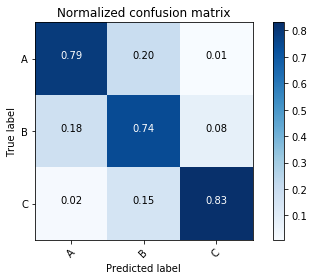
\includegraphics[width=.75\linewidth]{../Figures/conf_matrix_iter2.png} 
	\caption{Confusion matrix illustrating the performance of LR-BoW-Word model after augmentation}
	\label{fig:cmdstudy}
\end{figure}

\section {Conclusion}
\label{sec:conclusion}
In this paper, we have presented a classification method based on simple multinomial logistic regression and bag-of-words model augmented with semi-supervised (bootstrapping) method to classify English sentences based on their level difficulty, A=Beginner, B=intermediate, C=Advanced in accordancing. Our model achieves an overall F1 score of 0.69, and 0.79 after augmenting it with example sentences from unlabeled corpus. 
